\documentclass[xcolor=dvipsnames,t,compress]{beamer}
\usepackage{minted}

\setbeamersize{text margin left=5mm,text margin right=5mm}
\setminted{fontsize=\small,baselinestretch=1}

\usetheme{Frankfurt}
\usecolortheme{beaver}

\title{Basic Makefiles for Fun \& Profit}
\author{Ivan Sergeev}
\institute{\normalsize\texttt{git clone https://github.com/vsergeev/basic-makefiles.git}}
\date{May 2018}

\begin{document}

\frame{\titlepage}

\begin{frame}
\frametitle{Table of Contents}
\tableofcontents
\end{frame}

%%%%%%%%%%%%%%%%%%%%%%%%%%%%%%%%%%%%%%%%%%%%%%%%%%%%%%%%%%%%%%%%%%%%%%%%%%%%%%%%
% Introduction
%%%%%%%%%%%%%%%%%%%%%%%%%%%%%%%%%%%%%%%%%%%%%%%%%%%%%%%%%%%%%%%%%%%%%%%%%%%%%%%%

\section{Introduction}

\begin{frame}
\frametitle{What is make?}
A general-purpose tool to build outputs from inputs, following the rules specified in a Makefile.

\begin{itemize}[<+->]
\item Created for Unix by Stuart Feldman at Bell Labs, 1976
\item Often used for compilation, but is agnostic to objectives
\item GNU Make implementation is ubiquitous, and standard \\ on Linux and Mac OS X
\end{itemize}
\end{frame}

\begin{frame}[fragile]
\frametitle{Example of Running \texttt{make}}
Running \texttt{make} to build a small library project:
\\
\begin{minted}{shell}
$ make
cc -std=gnu99 -pedantic   -c -o gpio.o gpio.c
cc -std=gnu99 -pedantic   -c -o spi.o spi.c
cc -std=gnu99 -pedantic   -c -o i2c.o i2c.c
cc -std=gnu99 -pedantic   -c -o mmio.o mmio.c
cc -std=gnu99 -pedantic   -c -o serial.o serial.c
cc -std=gnu99 -pedantic   -c -o version.o version.c
ar rcs periphery.a gpio.o spi.o i2c.o mmio.o serial.o version.o
$ 
\end{minted}
\end{frame}

\begin{frame}
\frametitle{Why learn \texttt{make}? Automation}
\centering

\includegraphics[scale=0.5]{images/all-the-things-meme.jpg}
\end{frame}

\begin{frame}
\frametitle{Why learn \texttt{make}? Reincarnation}
\centering

\includegraphics[scale=0.4]{images/what-if-meme.jpg}
\end{frame}

\begin{frame}[fragile]
\frametitle{Example of a Makefile}
\vspace{-1.25em}
\begin{minted}{make}
LIB = periphery.a
SRCS = gpio.c spi.c i2c.c mmio.c serial.c version.c

CFLAGS += -std=gnu99 -pedantic
OBJECTS = $(patsubst %.c,%.o,$(SRCS))

.PHONY: all clean

all: $(LIB)

clean:
	-rm -f $(LIB) $(OBJECTS)

$(LIB): $(OBJECTS)
	ar rcs $(LIB) $(OBJECTS)

%.o: %.c
	$(CC) $(CFLAGS) $(LDFLAGS) -c $< -o $@
\end{minted}
\end{frame}

%%%%%%%%%%%%%%%%%%%%%%%%%%%%%%%%%%%%%%%%%%%%%%%%%%%%%%%%%%%%%%%%%%%%%%%%%%%%%%%%
% Example Problem
%%%%%%%%%%%%%%%%%%%%%%%%%%%%%%%%%%%%%%%%%%%%%%%%%%%%%%%%%%%%%%%%%%%%%%%%%%%%%%%%

\section{Example Problem}

\begin{frame}
\frametitle{Table of Contents}
\tableofcontents[currentsection]
\end{frame}

\begin{frame}
\frametitle{Wallpaper Gallery}
Let's automate building a static site for wallpapers.
\begin{center}
  \makebox[\textwidth]{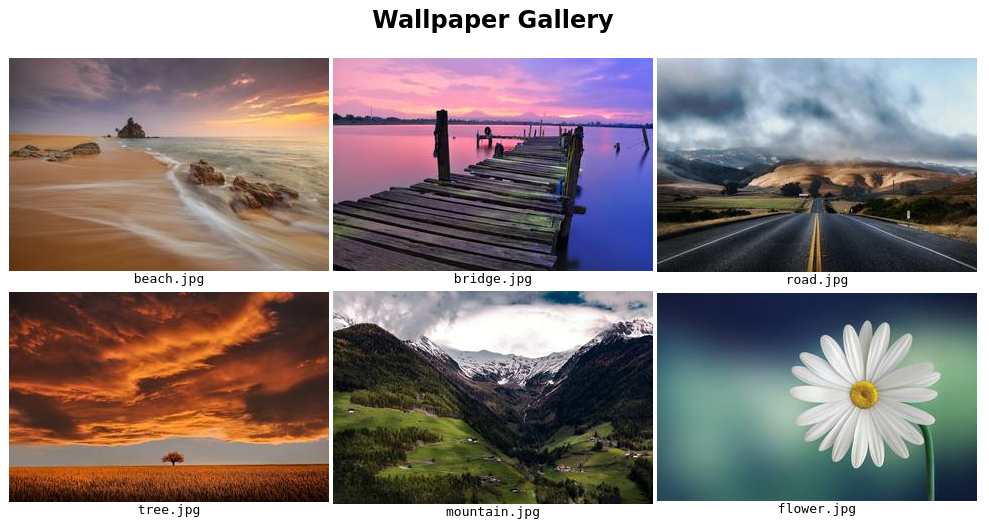
\includegraphics[width=\paperwidth]{images/gallery-6.png}}
\end{center}
\end{frame}

\begin{frame}[fragile]
\frametitle{File structure}
Project consists of wallpapers, a Python script, and a Mako template:
\\
\begin{minted}[escapeinside=||]{text}
$ ls
|\textcolor{PineGreen}{beach.jpg}|   |\textcolor{PineGreen}{flower.jpg}|    gallery.py     |\textcolor{PineGreen}{road.jpg}|
|\textcolor{PineGreen}{bridge.jpg}|  gallery.mako  |\textcolor{PineGreen}{mountain.jpg}|   |\textcolor{PineGreen}{tree.jpg}|
$
\end{minted}
\end{frame}

\begin{frame}[fragile]
\frametitle{Thumbnails}
We create 320 px thumbnails with ImageMagick's \texttt{convert}:
\\
\begin{minted}[escapeinside=||]{text}
$ convert -resize 320x beach.jpg beach.thumb.jpg
$ file beach.jpg beach.thumb.jpg
beach.jpg:       JPEG image data, JFIF standard 1.01,
                 resolution (DPI), density 72x72,
                 segment length 16, baseline,
                 precision 8, |\colorbox{yellow}{5616x3744}|, frames 3
beach.thumb.jpg: JPEG image data, JFIF standard 1.01,
                 resolution (DPI), density 72x72,
                 segment length 16, baseline,
                 precision 8, |\colorbox{yellow}{320x213}|, frames 3
$
\end{minted}
\end{frame}

\begin{frame}[fragile]
\frametitle{Python Script}
A Python script accepts the original images as arguments, and passes relevant information to a Mako template for rendering:
\\
\begin{minted}[escapeinside=||]{text}
$ python3 gallery.py beach.jpg bridge.jpg mountain.jpg
                     tree.jpg flower.jpg road.jpg > gallery.html
$ file gallery.html
gallery.html: HTML document, ASCII text
$
\end{minted}
\end{frame}

\begin{frame}[fragile]
\frametitle{Python Script}
\vspace{-1em}
\inputminted{py}{examples/script/gallery.py}
\end{frame}

\begin{frame}[fragile]
\frametitle{Gallery Template}
\vspace{-1em}
\inputminted{html}{examples/script/gallery.mako}
\end{frame}

\begin{frame}[fragile]
\frametitle{A Handcrafted, Artisanal Gallery}
\vspace{-1em}
\begin{minted}[escapeinside=||]{text}
$ convert -resize 320x beach.jpg beach.thumb.jpg
$ convert -resize 320x bridge.jpg bridge.thumb.jpg
$ convert -resize 320x mountain.jpg mountain.thumb.jpg
$ convert -resize 320x tree.jpg tree.thumb.jpg
$ convert -resize 320x flower.jpg flower.thumb.jpg
$ convert -resize 320x road.jpg road.thumb.jpg
$ python3 gallery.py beach.jpg bridge.jpg mountain.jpg
                     tree.jpg flower.jpg road.jpg > gallery.html
$
\end{minted}
Phew.
\end{frame}

\begin{frame}
\frametitle{Shell Script}
We could throw this all into a shell script, but we would still run into problems:
\begin{itemize}[<+->]
\item Scalability
\item Incremental builds
\item Maintainability
\end{itemize}
\pause
So let's use \texttt{make} instead.
\end{frame}

%%%%%%%%%%%%%%%%%%%%%%%%%%%%%%%%%%%%%%%%%%%%%%%%%%%%%%%%%%%%%%%%%%%%%%%%%%%%%%%%
% Basic Concepts
%%%%%%%%%%%%%%%%%%%%%%%%%%%%%%%%%%%%%%%%%%%%%%%%%%%%%%%%%%%%%%%%%%%%%%%%%%%%%%%%

\section{Basic Concepts}

\begin{frame}
\frametitle{Table of Contents}
\tableofcontents[currentsection]
\end{frame}

\begin{frame}[fragile]
\frametitle{Golden Rule}
\begin{block}{Anatomy of a Makefile Rule}
\begin{minted}[escapeinside=||,tabsize=4]{make}
target: dependencies...
	commands
	...
\end{minted}
\end{block}
\vspace{1em}
\begin{itemize}[<+->]
\item \texttt{make} executes a rule's \textbf{commands} to transform its \textbf{dependencies} into a \textbf{target}
\item If a dependency does not exist, \texttt{make} looks for and executes the rule responsible for creating it
\item \texttt{make} can be invoked to build specific target(s) with \\ \hspace{1em}\texttt{make [targets...]}
\item The first rule of a Makefile is the default target
\end{itemize}
\end{frame}

\begin{frame}[fragile]
\frametitle{Gotcha: Hard Tabs}
\vspace{-1em}
Commands in a Makefile rule must be indented with a \textbf{hard tab}! \\ Not spaces!

\begin{minted}[escapeinside=||,tabsize=4]{text}
$ cat Makefile
hello.txt:
|\colorbox{red}{\rule{0cm}{1.5ex}    }|echo "Hello World" > hello.txt
$ make
Makefile:2: *** missing separator.  Stop.
$

$ cat Makefile
hello.txt:
|\colorbox{green}{\rule{0cm}{1.5ex}	}|echo "Hello World" > hello.txt
$ make
echo "Hello World" > hello.txt
$
\end{minted}
\end{frame}

\begin{frame}[fragile]
\frametitle{Everything is a File}
\vspace{-0.75em}
\begin{minted}[tabsize=4,frame=single]{make}
beach.thumb.jpg: beach.jpg
	convert -resize 320x beach.jpg beach.thumb.jpg
\end{minted}
In \texttt{make}, every target and dependency is simply a file.
\pause
\vspace{0.25em}
\begin{minted}[escapeinside=||,tabsize=4]{text}
$ make beach.thumb.jpg
convert -resize 320x beach.jpg beach.thumb.jpg
$
$ make beach.thumb.jpg
make: Nothing to be done for 'beach.thumb.jpg'.
$
\end{minted}
Once the target exists, there is no need to re-execute the rule. *
\end{frame}


\begin{frame}[fragile]
\frametitle{Starting small}
Let's put together a Makefile to generate the static gallery with two images:
\inputminted[tabsize=4,frame=single]{make}{examples/make/Makefile.2}
\pause
\begin{minted}[escapeinside=||,tabsize=4]{text}
$ make
convert -resize 320x beach.jpg beach.thumb.jpg
convert -resize 320x bridge.jpg bridge.thumb.jpg
python3 gallery.py beach.jpg bridge.jpg > gallery.html
$
\end{minted}
\end{frame}

\begin{frame}[fragile]
\frametitle{Breaking it down}
\vspace{-1em}
\begin{minted}[tabsize=4,frame=single,escapeinside=||]{text}
|\colorbox{BrickRed}{gallery.html}|: |\colorbox{SeaGreen}{beach.jpg}| |\colorbox{SeaGreen}{bridge.jpg}|
              |\colorbox{BrickRed}{beach.thumb.jpg}| |\colorbox{BrickRed}{bridge.thumb.jpg}| \
			  |\colorbox{SeaGreen}{gallery.mako}| |\colorbox{SeaGreen}{gallery.py}|
	python3 gallery.py beach.jpg bridge.jpg > gallery.html

beach.thumb.jpg: beach.jpg
	convert -resize 320x beach.jpg beach.thumb.jpg

bridge.thumb.jpg: bridge.jpg
	convert -resize 320x bridge.jpg bridge.thumb.jpg
\end{minted}
\begin{minted}[escapeinside=||,tabsize=4]{text}
$ make
\end{minted}
\end{frame}

\begin{frame}[fragile]
\frametitle{Breaking it down}
\vspace{-1em}
\begin{minted}[tabsize=4,frame=single,escapeinside=||]{text}
|\colorbox{BrickRed}{gallery.html}|: |\colorbox{SeaGreen}{beach.jpg}| |\colorbox{SeaGreen}{bridge.jpg}|
              |\colorbox{BrickRed}{beach.thumb.jpg}| |\colorbox{BrickRed}{bridge.thumb.jpg}| \
			  |\colorbox{SeaGreen}{gallery.mako}| |\colorbox{SeaGreen}{gallery.py}|
	python3 gallery.py beach.jpg bridge.jpg > gallery.html

|\colorbox{BrickRed}{beach.thumb.jpg}|: |\colorbox{SeaGreen}{beach.jpg}|
	|\colorbox{ProcessBlue}{convert -resize 320x beach.jpg beach.thumb.jpg}|

bridge.thumb.jpg: bridge.jpg
	convert -resize 320x bridge.jpg bridge.thumb.jpg
\end{minted}
\begin{minted}[escapeinside=||,tabsize=4]{text}
$ make
convert -resize 320x beach.jpg beach.thumb.jpg
\end{minted}
\end{frame}

\begin{frame}[fragile]
\frametitle{Breaking it down}
\vspace{-1em}
\begin{minted}[tabsize=4,frame=single,escapeinside=||]{text}
|\colorbox{BrickRed}{gallery.html}|: |\colorbox{SeaGreen}{beach.jpg}| |\colorbox{SeaGreen}{bridge.jpg}|
              |\colorbox{SeaGreen}{beach.thumb.jpg}| |\colorbox{BrickRed}{bridge.thumb.jpg}| \
			  |\colorbox{SeaGreen}{gallery.mako}| |\colorbox{SeaGreen}{gallery.py}|
	python3 gallery.py beach.jpg bridge.jpg > gallery.html

beach.thumb.jpg: beach.jpg
	convert -resize 320x beach.jpg beach.thumb.jpg

bridge.thumb.jpg: bridge.jpg
	convert -resize 320x bridge.jpg bridge.thumb.jpg
\end{minted}
\begin{minted}[escapeinside=||,tabsize=4]{text}
$ make
convert -resize 320x beach.jpg beach.thumb.jpg
\end{minted}
\end{frame}

\begin{frame}[fragile]
\frametitle{Breaking it down}
\vspace{-1em}
\begin{minted}[tabsize=4,frame=single,escapeinside=||]{text}
|\colorbox{BrickRed}{gallery.html}|: |\colorbox{SeaGreen}{beach.jpg}| |\colorbox{SeaGreen}{bridge.jpg}|
              |\colorbox{SeaGreen}{beach.thumb.jpg}| |\colorbox{BrickRed}{bridge.thumb.jpg}| \
			  |\colorbox{SeaGreen}{gallery.mako}| |\colorbox{SeaGreen}{gallery.py}|
	python3 gallery.py beach.jpg bridge.jpg > gallery.html

beach.thumb.jpg: beach.jpg
	convert -resize 320x beach.jpg beach.thumb.jpg

|\colorbox{BrickRed}{bridge.thumb.jpg}|: |\colorbox{SeaGreen}{bridge.jpg}|
	|\colorbox{ProcessBlue}{convert -resize 320x bridge.jpg bridge.thumb.jpg}|
\end{minted}
\begin{minted}[escapeinside=||,tabsize=4]{text}
$ make
convert -resize 320x beach.jpg beach.thumb.jpg
convert -resize 320x bridge.jpg bridge.thumb.jpg
\end{minted}
\end{frame}

\begin{frame}[fragile]
\frametitle{Breaking it down}
\vspace{-1em}
\begin{minted}[tabsize=4,frame=single,escapeinside=||]{text}
|\colorbox{BrickRed}{gallery.html}|: |\colorbox{SeaGreen}{beach.jpg}| |\colorbox{SeaGreen}{bridge.jpg}|
              |\colorbox{SeaGreen}{beach.thumb.jpg}| |\colorbox{SeaGreen}{bridge.thumb.jpg}| \
			  |\colorbox{SeaGreen}{gallery.mako}| |\colorbox{SeaGreen}{gallery.py}|
	|\colorbox{ProcessBlue}{python3 gallery.py beach.jpg bridge.jpg > gallery.html}|

beach.thumb.jpg: beach.jpg
	convert -resize 320x beach.jpg beach.thumb.jpg

bridge.thumb.jpg: bridge.jpg
	convert -resize 320x bridge.jpg bridge.thumb.jpg
\end{minted}
\begin{minted}[escapeinside=||,tabsize=4]{text}
$ make
convert -resize 320x beach.jpg beach.thumb.jpg
convert -resize 320x bridge.jpg bridge.thumb.jpg
python3 gallery.py beach.jpg bridge.jpg > gallery.html
$
\end{minted}
\end{frame}

\begin{frame}[fragile]
\frametitle{Two image gallery, output}
\begin{center}
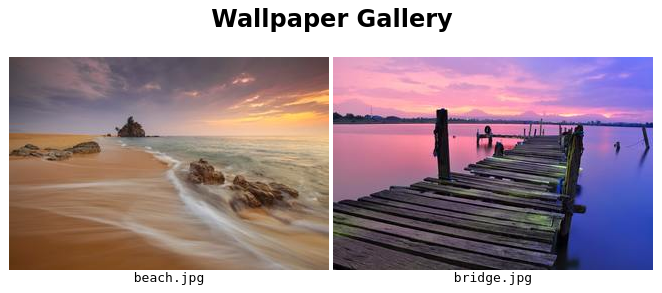
\includegraphics[scale=0.4]{images/gallery-2.png}
\end{center}
\end{frame}

\begin{frame}[fragile]
\frametitle{Simplifying Rules}
\vspace{-0.75em}
\begin{minted}[tabsize=4,frame=single]{make}
beach.thumb.jpg: beach.jpg
	convert -resize 320x beach.jpg beach.thumb.jpg

bridge.thumb.jpg: bridge.jpg
	convert -resize 320x bridge.jpg bridge.thumb.jpg
\end{minted}
\pause
\texttt{make} exposes useful \textbf{automatic variables} to the commands of rules:
\begin{itemize}
\item \texttt{\$@} - the target
\item \texttt{\$<} - the first dependency
\item \texttt{\$\^} - all of the dependencies
\end{itemize}
\pause
\vspace{0.5em}
We can avoid repetition by using these instead of explicit names:
\begin{minted}[tabsize=4,frame=single]{make}
beach.thumb.jpg: beach.jpg
	convert -resize 320x $< $@

bridge.thumb.jpg: bridge.jpg
	convert -resize 320x $< $@
\end{minted}
\end{frame}

\begin{frame}[fragile]
\frametitle{Two image gallery, Makefile, rewritten}
\vspace{-1em}
\inputminted[frame=single,tabsize=4]{make}{examples/make/Makefile.3}
\end{frame}

\begin{frame}[fragile]
\frametitle{Rule Sprawl}
\vspace{-0.75em}
\begin{minted}[tabsize=4,frame=single]{make}
beach.thumb.jpg: beach.jpg
	convert -resize 320x $< $@

bridge.thumb.jpg: bridge.jpg
	convert -resize 320x $< $@
\end{minted}
At this point, we have fairly generic rule bodies, but a lot of duplication for each target.
\end{frame}

\begin{frame}[fragile]
\frametitle{Pattern Rules}
\vspace{-0.75em}
Fortunately, \texttt{make} supports a simple form of pattern matching with \textbf{pattern rules}:
\begin{itemize}
\item \texttt{\%} is the pattern match placeholder
\item \texttt{\%} matches one or more character
\item \texttt{\%} can be used in the target and the dependencies
\end{itemize}
\pause
\vspace{0.5em}
We can rewrite our rules for thumbnail generation to be completely generic:
\begin{minted}[tabsize=4,frame=single]{make}
%.thumb.jpg: %.jpg
	convert -resize 320x $< $@
\end{minted}
\end{frame}

\begin{frame}[fragile]
\frametitle{Two image gallery, Makefile, rewritten}
\vspace{-1em}
\inputminted[fontsize=\small,frame=single,tabsize=4]{make}{examples/make/Makefile.4}
\begin{minted}[fontsize=\small,escapeinside=||,tabsize=4]{text}
$ make
convert -resize 320x beach.jpg beach.thumb.jpg
convert -resize 320x bridge.jpg bridge.thumb.jpg
python3 gallery.py beach.jpg bridge.jpg > gallery.html
$
\end{minted}
\end{frame}

\begin{frame}[fragile]
\frametitle{Incremental Builds}
\vspace{-0.75em}
By the way, what happens if we change a deeply buried dependency?

\begin{minted}[fontsize=\small,escapeinside=||,tabsize=4]{text}
$ cp ~/better-beach.jpg beach.jpg|\pause|
$ make
convert -resize 320x beach.jpg beach.thumb.jpg
python3 gallery.py beach.jpg bridge.jpg > gallery.html
$
\end{minted}

\texttt{make} only rebuilds the targets that were dependent on \texttt{beach.jpg}, and not the targets associated with \texttt{bridge.jpg}.
\\
\newline
How does it know?
\end{frame}


\begin{frame}[fragile]
\frametitle{Incremental Builds}
\vspace{-1em}
\texttt{make} will re-execute a rule when a dependency's \textbf{modified time} is newer than that of the target.
\\
\newline
We can check the \textbf{mtime} of files with the \texttt{stat} command:
\begin{minted}[fontsize=\scriptsize,escapeinside=||,tabsize=4]{text}
$ stat bridge.jpg
  File: bridge.jpg
  Size: 1594290   	Blocks: 3120       IO Block: 4096   regular file
  ...
Modify: 2018-05-24 01:29:19.459575114 -0500
  ...
  File: bridge.thumb.jpg
  Size: 14485     	Blocks: 32         IO Block: 4096   regular file
  ...
Modify: 2018-05-24 04:45:10.815519021 -0500
  ...
$
\end{minted}
\end{frame}

\begin{frame}[fragile]
\frametitle{Incremental Builds}
\vspace{-1em}
We can fool \texttt{make} into rebuilding targets associated with \texttt{bridge.jpg} by updated its mtime with \texttt{touch}:
\begin{minted}[fontsize=\scriptsize,escapeinside=||,tabsize=4]{text}
$ make
make: 'gallery.html' is up to date.
$|\pause| touch -m bridge.jpg
$|\pause| stat bridge.jpg
  File: bridge.jpg
  Size: 1594290   	Blocks: 3120       IO Block: 4096   regular file
  	...
Modify: 2018-05-24 05:06:33.815877712 -0500
 Birth: -
  File: bridge.thumb.jpg
  Size: 14485     	Blocks: 32         IO Block: 4096   regular file
  	...
Modify: 2018-05-24 04:45:10.815519021 -0500
	...
$|\pause| make
convert -resize 320x bridge.jpg bridge.thumb.jpg
python3 gallery.py beach.jpg bridge.jpg > gallery.html
$
\end{minted}
\end{frame}

\begin{frame}[fragile]
\frametitle{Using Variables}
\vspace{-1em}
\texttt{make} supports simple string variables.
\begin{itemize}
\item Can be scalars or space-delimited lists
\item Defined with \texttt{FOO = text}
\item Expanded with \texttt{\$(FOO)}
\end{itemize}
\pause
\vspace{1em}
We can define variables for our inputs and parameters:
\begin{minted}[fontsize=\small,escapeinside=||,tabsize=4]{make}
IMAGE_FILES = beach.jpg bridge.jpg
THUMB_FILES = beach.thumb.jpg bridge.thumb.jpg
THUMB_WIDTH = 320
OUTPUT = gallery.html
\end{minted}
and expand them with \texttt{\$(IMAGE\_FILES)}, \texttt{\$(THUMB\_FILES)}, \texttt{\$(THUMB\_WIDTH)}, \texttt{\$(OUTPUT)}.
\end{frame}

\begin{frame}[fragile]
\frametitle{Two image gallery, Makefile, rewritten}
\vspace{-1em}
\inputminted[fontsize=\small,frame=single,tabsize=4]{make}{examples/make/Makefile.5}
\end{frame}

\begin{frame}[fragile]
\frametitle{Clean up on aisle \texttt{\$PWD}}
\vspace{-1em}
Our working directory has become quite a mess:
\begin{minted}[escapeinside=||]{text}
$ ls
|\textcolor{PineGreen}{beach.jpg}|        |\textcolor{PineGreen}{bridge.thumb.jpg}|  gallery.mako  |\textcolor{PineGreen}{mountain.jpg}|
|\textcolor{PineGreen}{beach.thumb.jpg}|  |\textcolor{PineGreen}{flower.jpg}|        gallery.py    |\textcolor{PineGreen}{road.jpg}|
|\textcolor{PineGreen}{bridge.jpg}|       gallery.html      Makefile      |\textcolor{PineGreen}{tree.jpg}|
$
\end{minted}
\pause
\vspace{1em}
It's a common convention to include abstract targets, called \textbf{goals}, like \texttt{all}, \texttt{clean}, or \texttt{install}, to accomplish certain tasks.
\begin{minted}[fontsize=\small,escapeinside=||,tabsize=4]{make}
clean:
	rm $(THUMB_FILES) $(OUTPUT)
\end{minted}
\begin{minted}[escapeinside=||,tabsize=4]{text}
$ make clean
rm beach.thumb.jpg bridge.thumb.jpg gallery.html
$
\end{minted}
\end{frame}

\begin{frame}[fragile]
\frametitle{Two image gallery, Makefile, rewritten}
\vspace{-1em}
\inputminted[fontsize=\small,frame=single,tabsize=4]{make}{examples/make/Makefile.6}
\end{frame}

\begin{frame}[fragile]
\frametitle{Gotcha: Exit Codes}
However, one thing to keep in mind is that \texttt{make} uses \textbf{exit codes} to detect failure when executing a rule.
\begin{minted}[fontsize=\small,escapeinside=||]{text}
$ make clean
rm beach.thumb.jpg bridge.thumb.jpg gallery.html
$ make clean
rm beach.thumb.jpg bridge.thumb.jpg gallery.html
rm: cannot remove 'beach.thumb.jpg': No such file or directory
rm: cannot remove 'bridge.thumb.jpg': No such file or directory
rm: cannot remove 'gallery.html': No such file or directory
make: *** [Makefile.6:11: clean] Error 1
$
\end{minted}
\pause
We can ask \texttt{make} to ignore the failure of a command by prefixing it with a dash \texttt{-} character, so it will continue executing the next command or target.
\\
\newline
In this case, it's common to use \texttt{rm -f} to surpress errors altogether.
\end{frame}

\begin{frame}[fragile]
\frametitle{Two image gallery, Makefile, rewritten}
\vspace{-1em}
\inputminted[fontsize=\small,frame=single,tabsize=4]{make}{examples/make/Makefile.7}
\end{frame}


%%%%%%%%%%%%%%%%%%%%%%%%%%%%%%%%%%%%%%%%%%%%%%%%%%%%%%%%%%%%%%%%%%%%%%%%%%%%%%%%
% Intermediate Concepts
%%%%%%%%%%%%%%%%%%%%%%%%%%%%%%%%%%%%%%%%%%%%%%%%%%%%%%%%%%%%%%%%%%%%%%%%%%%%%%%%

\section{Intermediate Concepts}

\begin{frame}[fragile]
\frametitle{Those .PHONY targets}
\vspace{-1em}
What happened to everything is a file? Don't worry, everything still is.
\begin{minted}[fontsize=\footnotesize,escapeinside=||]{text}
$ echo "hello world" > clean
$ cat clean
hello world
$ make clean
make: Nothing to be done for 'clean'.
$
\end{minted}
\pause
In order for rules with goals or other file-less targets to always execute, we need to mark them \texttt{.PHONY}:
\begin{minted}[fontsize=\footnotesize,escapeinside=||,tabsize=4]{make}
.PHONY: clean
clean:
	rm $(THUMB_FILES) $(OUTPUT)
\end{minted}
\begin{minted}[fontsize=\footnotesize,escapeinside=||]{text}
$ cat clean
hello world
$ make clean
rm beach.thumb.jpg bridge.thumb.jpg gallery.html
$
\end{minted}
\end{frame}

\begin{frame}[fragile]
\frametitle{Two image gallery, Makefile, rewritten}
\vspace{-1em}
\inputminted[fontsize=\footnotesize,frame=single,tabsize=4]{make}{examples/make/Makefile.8}
\end{frame}

\begin{frame}[fragile]
\frametitle{Using \texttt{\$(patsubst ...)}}
\vspace{-1em}
Our \texttt{\$(THUMB\_FILES)} variable is essentially a permutation of the input \texttt{\$(IMAGE\_FILES)} variable.
\begin{minted}[fontsize=\small,escapeinside=||,tabsize=4]{make}
IMAGE_FILES = beach.jpg bridge.jpg
THUMB_FILES = beach.thumb.jpg bridge.thumb.jpg
\end{minted}
\pause
\vspace{1em}
We can use the powerful \texttt{\$(patsubst \textit{pattern},\textit{replacement},\textit{text})} function to generate it.
\begin{minted}[fontsize=\small,escapeinside=||,tabsize=4]{make}
IMAGE_FILES = beach.jpg bridge.jpg
THUMB_FILES = $(patsubst %.jpg,%.thumb.jpg,$(IMAGE_FILES))
\end{minted}
The \texttt{\%} is used as a wildcard in the pattern and replacement, much like in pattern rules.
\end{frame}

\begin{frame}[fragile]
\frametitle{Two image gallery, Makefile, rewritten}
\vspace{-1em}
\inputminted[fontsize=\footnotesize,frame=single,tabsize=4]{make}{examples/make/Makefile.9}
\end{frame}

\begin{frame}[fragile]
\frametitle{Adding a \texttt{dist/} folder}
\vspace{-1em}
Often, we want to consolidate build products to a folder, e.g. website deployment. \\
\newline
We can model the \texttt{dist} folder like any other target or dependency:
\begin{minted}[escapeinside=||,tabsize=4]{make}
OUTPUT_DIR = dist

$(OUTPUT_DIR):
	mkdir $@
\end{minted}
\vspace{1em}
And create an additional rule to copy the images to the \texttt{dist} folder:
\begin{minted}[escapeinside=||,tabsize=4]{make}
$(OUTPUT_DIR)/%.jpg: %.jpg $(OUTPUT_DIR)
	cp $< $@
\end{minted}
\end{frame}

\begin{frame}[fragile]
\frametitle{Two image gallery, Makefile, rewritten 1/2}
\vspace{-1em}
\inputminted[fontsize=\small,frame=single,tabsize=4,firstline=1,lastline=12]{make}{examples/make/Makefile.10}
\end{frame}

\begin{frame}[fragile]
\frametitle{Two image gallery, Makefile, rewritten 2/2}
\vspace{-1em}
\inputminted[fontsize=\small,frame=single,tabsize=4,firstline=13,lastline=24]{make}{examples/make/Makefile.10}
\end{frame}

\begin{frame}[fragile]
\frametitle{A slight problem...}
\vspace{-1em}
Everything seems to work on the surface. But, if we run \texttt{make} twice:

\begin{minted}[fontsize=\scriptsize,escapeinside=||]{text}
$ make
mkdir dist
cp beach.jpg dist/beach.jpg
cp bridge.jpg dist/bridge.jpg
convert -resize 320x beach.jpg dist/beach.thumb.jpg
convert -resize 320x bridge.jpg dist/bridge.thumb.jpg
python3 gallery.py beach.jpg bridge.jpg > dist/gallery.html
$ make
cp beach.jpg dist/beach.jpg
cp bridge.jpg dist/bridge.jpg
convert -resize 320x beach.jpg dist/beach.thumb.jpg
convert -resize 320x bridge.jpg dist/bridge.thumb.jpg
python3 gallery.py beach.jpg bridge.jpg > dist/gallery.html
$
\end{minted}
\texttt{make} is always rebuilding all the targets that have the folder as a dependency.
\pause
\\
This is because the \texttt{dist} folder itself has a modified time, which will be updated any time a file within it changes.
\end{frame}

\begin{frame}[fragile]
\frametitle{"Order-only" Dependencies}
`make` has a special syntax to separate dependencies that should not be time tracked, called "order-only" dependencies:
\begin{block}{Anatomy of a Makefile Rule}
\begin{minted}[escapeinside=||,tabsize=4]{text}
target: dependencies... | order-only dependencies...
	commands
	...
\end{minted}
\end{block}
\vspace{1em}
We can annotate the rules that depend on the \texttt{dist} folder with the pipe \texttt{|} symbol separator.
\end{frame}

\begin{frame}[fragile]
\frametitle{Two image gallery, Makefile, rewritten 1/2}
\vspace{-1em}
\inputminted[fontsize=\small,frame=single,tabsize=4,firstline=1,lastline=12]{make}{examples/make/Makefile.11}
\end{frame}

\begin{frame}[fragile]
\frametitle{Two image gallery, Makefile, rewritten 2/2}
\vspace{-1em}
\inputminted[fontsize=\small,frame=single,tabsize=4,firstline=13,lastline=24]{make}{examples/make/Makefile.11}
\end{frame}

\begin{frame}[fragile]
\frametitle{Scaling up with \texttt{\$(wildcard ...)}}
\vspace{-1em}
With the help of the function \texttt{\$(wildcard ...)}, we can extend our Makefile to automatically include all images.

\begin{minted}[escapeinside=||,tabsize=4]{make}
IMAGES := $(wildcard *.jpg)
\end{minted}
\begin{itemize}
\item \texttt{:=} indicates immediate expansion, so the wildcard isn't evaluated multiple times in the Makefile.
\item \texttt{make} features countless other functions useful for building target lists: \texttt{\$(shell ...)}, \texttt{\$(basename ...)}, \texttt{\$(dir ...)}, etc.
\end{itemize}
\end{frame}

\begin{frame}[fragile]
\frametitle{Full image gallery, Makefile, rewritten 1/2}
\vspace{-1em}
\inputminted[fontsize=\small,frame=single,tabsize=4,firstline=1,lastline=15]{make}{examples/final/Makefile}
\end{frame}

\begin{frame}[fragile]
\frametitle{Full image gallery, Makefile, rewritten 2/2}
\vspace{-1em}
\inputminted[fontsize=\small,frame=single,tabsize=4,firstline=16,lastline=27]{make}{examples/final/Makefile}
\end{frame}

\begin{frame}[fragile]
\frametitle{When everything has to be a file... create them?}
\vspace{-1em}
\begin{itemize}[<+->]
\item Sometimes, a build step mutates existing files (like a patch, append, etc.) and doesn't create a new one.
\item \texttt{make} can't track these steps, as it only understands a target is met with a file.
\item Idiomatic to create a dummy a "stamp" file marking the completion of that step.
\end{itemize}
\pause
\begin{minted}[tabsize=4]{make}
secret.txt: data.txt
    rm -f $@
    cat $< | tr 'A-Za-z' 'N-ZA-Mn-za-m' > $@

permissions-stamp: secret.txt
    chmod 600 $<
    touch $@
\end{minted}
\end{frame}

%%%%%%%%%%%%%%%%%%%%%%%%%%%%%%%%%%%%%%%%%%%%%%%%%%%%%%%%%%%%%%%%%%%%%%%%%%%%%%%%
% Conclusion
%%%%%%%%%%%%%%%%%%%%%%%%%%%%%%%%%%%%%%%%%%%%%%%%%%%%%%%%%%%%%%%%%%%%%%%%%%%%%%%%

\section{Conclusion}

\begin{frame}[fragile]
\frametitle{Final Makefile 1/2}
\vspace{-1em}
\inputminted[fontsize=\small,frame=single,tabsize=4,firstline=1,lastline=15]{make}{examples/final/Makefile}
\end{frame}

\begin{frame}[fragile]
\frametitle{Final Makefile 2/2}
\vspace{-1em}
\inputminted[fontsize=\small,frame=single,tabsize=4,firstline=16,lastline=27]{make}{examples/final/Makefile}
\end{frame}

\begin{frame}[fragile]
\frametitle{Final Build}
\begin{minted}[fontsize=\small]{shell}
$ make
mkdir dist
cp mountain.jpg dist/mountain.jpg
cp beach.jpg dist/beach.jpg
cp bridge.jpg dist/bridge.jpg
cp flower.jpg dist/flower.jpg
cp road.jpg dist/road.jpg
cp tree.jpg dist/tree.jpg
convert -resize 320x mountain.jpg dist/mountain.thumb.jpg
convert -resize 320x beach.jpg dist/beach.thumb.jpg
convert -resize 320x bridge.jpg dist/bridge.thumb.jpg
convert -resize 320x flower.jpg dist/flower.thumb.jpg
convert -resize 320x road.jpg dist/road.thumb.jpg
convert -resize 320x tree.jpg dist/tree.thumb.jpg
python3 gallery.py beach.jpg bridge.jpg road.jpg
                   tree.jpg mountain.jpg flower.jpg
				   > dist/gallery.html
$
\end{minted}
\end{frame}

\begin{frame}
\frametitle{Result}
\begin{center}
  \makebox[\textwidth]{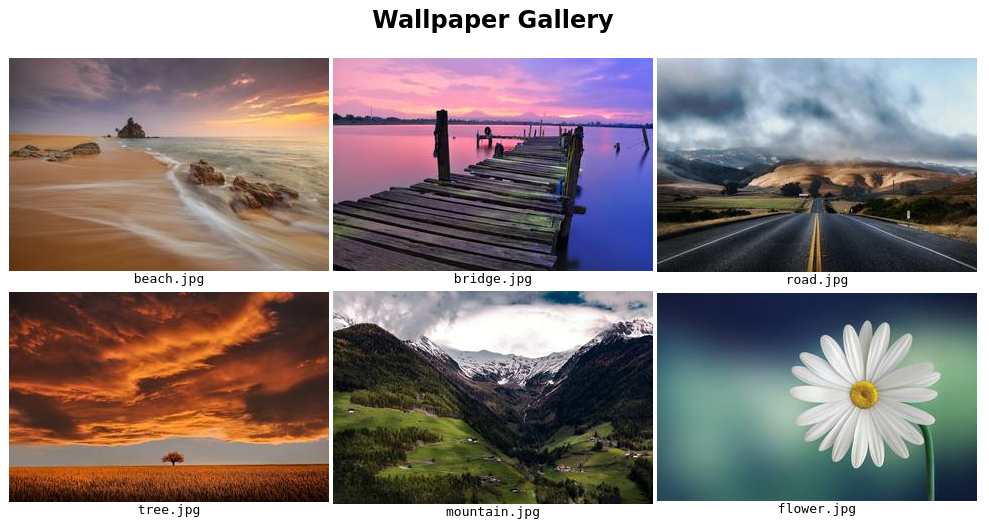
\includegraphics[width=\paperwidth]{images/gallery-6.png}}
\end{center}
\end{frame}

\begin{frame}
\frametitle{Limitations of Make}
\begin{itemize}[<+->]
\item Manual dependency grap
\item Everything is a file
\item Shell commands
\end{itemize}
\end{frame}

\begin{frame}
\frametitle{Should you use make?}
\begin{itemize}[<+->]
\item Maybe
\begin{itemize}
\item Slightly more complicated than a shell script? Yes
\item Building C/C++? Probably
\item Some hipster language with a built-in build system? No
\end{itemize}
\item Inevitably
\begin{itemize}
\item You may find yourself automating other build tools\ldots
\end{itemize}
\end{itemize}
\end{frame}

\begin{frame}
\frametitle{Questions}
\begin{center}
\Huge Questions?
\end{center}
\end{frame}

\end{document}
